\chapter{Conception}
This chapter describes the concept and design of the application based on the previously analyzed requirements. This chapter outlines the application's structure, functionalities, technologies, and patterns used to fulfill the listed requirements.

\section{System Architecture}
In this section, an architecture diagram is displayed to have a better understanding of the system architecture as well as its components.
\begin{figure}[H]
    \centering
    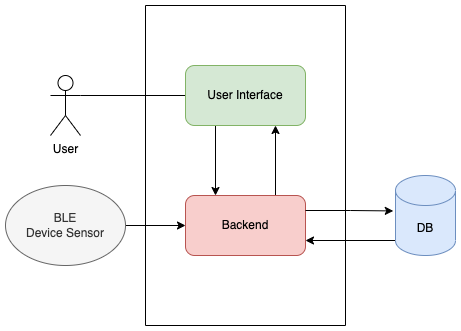
\includegraphics[width=1\textwidth]{diagrams/system-diagram.drawio.png}
    \caption{System architecture diagram}
    \label{fig:sys_diagram}
\end{figure}
\autoref{fig:sys_diagram} illustrates the components of the systems and the interaction between the components. Within the system, there are two components: the user interface and the backend which connects to a local database to store and manage data.
In addition, the device sensor is connected to the backend via bluetooth low energy and transmit the user's heart rate.
\section{Software Architecture}
This section serves as a guide to the high level structure of the application. It defines the key components as well as their relationship with each other.
Moreover, it describes the fundamental design patterns and architecture that define the application and its functionalities. 
The diagram presented below helps to gain better understanding of the application's architecture.
\begin{figure}[H]
    \centering
    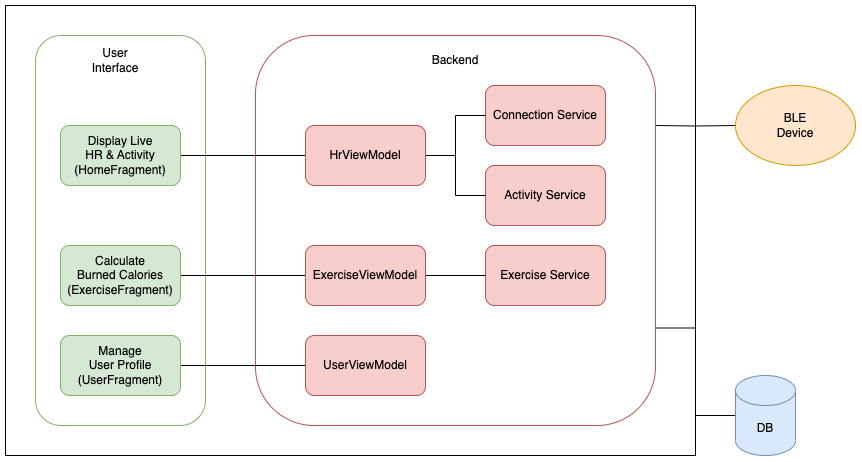
\includegraphics[width=1\textwidth]{diagrams/architecture-diagram.drawio.png}
    \caption{Software architecture diagram}
    \label{fig:soft_diagram}
\end{figure}
The project follows the Model-View-ViewModel (MVVM) architectural pattern. The user interface, which is responsible for displaying the features to the user, represents the \emph{view}. 
The \emph{model} is represented by the data and the business logic of the application, for instance, the entities and the functionalities such as live heart rate monitor, activity monitoring, exercise service, and user data management. 
The \emph{view model} facilitate the communications between the \emph{models} and the \emph{views} through which the \emph{views} can access and interact with the data and operations of the \emph{models}.

The user interface consists of three main components which extends \texttt{Fragment}\footnote{Based on The Official Android Documentation, a Fragment represents a reusable portion of your app's UI. A fragment defines and manages its own layout, has its own lifecycle, and can handle its own input events. \autocite{android-fragments}}. 
The \texttt{HomeFragment} displays real-time heart rate data and the activity monitor. It serves as the initial entry point for the users as they log in to the application. As it shows live heart rate data and activity, it holds a connection to the \texttt{HrViewModel}.
The \texttt{ExerciseFragment} presents the number of calories burned in an exercise based on the user's heart rate. It maintains a connection with the \texttt{ExerciseViewModel}. Lastly, the \texttt{UserFragment}, which is connected to the \texttt{UserViewModel}, displays the user's data and provide the necessary UI components to support data management.

The backend is in charge of the core functionalities of the application, which involve establishing a connection to the database.
As one of the core components, the \texttt{ConnectionService} maintains the connection between the BLE device and the application. It actively listens to the heart rate data being broadcasted by the BLE device. 
The \texttt{ActivityService} determines the current activity status based on the user's heart rate and age. 
On the other hand, the \texttt{ExerciseService} tracks the user's energy expenditure during training based on the user's heart rate and physical measurements such as weight, age, and gender. Both the \texttt{ExerciseService} and \texttt{ActivityService} subscribe to an event, where the heart rate data is published by the \texttt{ConnectionService}. This enables the services to receive the heart rate data seamlessly and process it accordingly.
Lastly, the \texttt{UserViewModel} is responsible for the management of the user's data and facilitates CRUD operations related to the user's data.

\section{Technologies}
\label{chap:tech}
This section provides an overview of the key technologies required to develop the application. 
The goal of this phase is to find the most suitable technologies based on the goal of this project and preferences of the writer. 
Android with Kotlin is chosen as the development platform for this project due to its widespread popularity and compatibility with the Model-View-ViewModel architectural pattern. Additionally, Android offers a wide range of development tools and resources, making it suitable for this project.

\subsection{User Interface}
As the main development platform for this project is Android Kotlin, the user interface is designed and implemented using a combination of Kotlin and XML with the help of Material Design\footnote{\emph{Material Design} is a design language developed by Google. Homepage: \url{https://m2.material.io/develop/android}}.
Implementing a graph to display live heart rate data can be advantageous to the user. Therefore, for smooth and appealing visualization, MPAndroidChart\footnote{\emph{MPAndroidChart} is a chart library for Android, designed for generating interactive and dynamic charts. Github repository: \url{https://github.com/PhilJay/MPAndroidChart}} is used to help with the graph implementation.
\subsection{Backend Infrastructure}
As mentioned before, the backend of the application is developed using Kotlin with Android Jetpack\footnote{\emph{Jetpack} is a suite of libraries, tools, and guidance to help developers write apps easier. URL: \url{https://developer.android.com/jetpack}} due to its compatibility with the MVVM architecture. 
Furthermore, Kotlin provides pre-defined classes such as the \emph{Service}\footnote{Based on The Official Android Documentation, \emph{Service} is an application component that can perform long-running operations in the background.\autocite{android-services}} class, which enables smooth execution of long running task. In the scope of this project, \emph{Service} class is especially useful to implement the \texttt{ConnectionService} and \texttt{ExerciseService}.

\subsection{Database}
A database is required to store and manage data. In the context of this project, ROOM\footnote{\emph{ROOM} is a persistence library that provides an abstraction layer over SQLite to allow for more robust database access while harnessing the full power of SQLite. URL: \url{https://developer.android.com/jetpack/androidx/releases/room}} database, which is built on top of SQLite\footnote{\emph{SQLite} is a C-language library that implements a small, fast, self-contained, high-reliability, full-featured, SQL database engine. Homepage: \url{https://www.sqlite.org/index.html}} has been selected as the application's database.

\subsection{BLE Sensor Device}
Once all the technologies required to develop the application have been decided, the next step is to select a suitable heart-rate sensor device. Considering factors like accuracy, performance, and affordability, Polar H9\footnote{\emph{Polar H9} is a heart rate sensor made by Polar. Homepage: \url{https://www.polar.com/en/sensors/h9-heart-rate-sensor}} is chosen as the preferred device due to its affordability and reputation for providing reliable heart-rate measurements and long battery life.




\section{Software Design}
the model-view-viewmodel follows the separation of concerns principles blablabla
The MVVM pattern promotes loose coupling and separation of concerns, making the application more maintainable and testable. The View and ViewModel are often connected using data binding techniques, allowing automatic synchronization of data between the two.
By following MVVM, developers can achieve a clear separation of responsibilities, allowing for easier development, testing, and maintenance of the application.
\subsection{Model}
\subsection{View}
\subsection{ViewModel}

% \section{Features}
